\clearpage
\section{Installation Sprach Assistant} \label{sec:Assistant}
Der Home Assistant ist die Schnittstelle, welche den Google Assistant mit Openhab verbindet. Die Kommunikation zwischen Homeassistant und Openhab findet über MQTT statt. Die Homeassistant Software wird auf ein weiteres Rasberrypi installiert. Die Verbindung zwischen Home Assistant und Google Assistant Basiert auf einer Öffentlichen Cloud gemäss Abbildung \ref{pic: Systemübersicht}.

\begin{enumerate}
	\item Download des Images für die Installation auf dem eigenen Raspi von der offiziellen Home Assistant \cite{assistant_installing_nodate} Webseite.
\item Image auf Micro SD-Card mit balenaEtcher \cite{noauthor_balenaetcher_nodate} schreiben. 
\item Ein USB-Stick, FAT32 formatieren und ihn als 'CONFIG' benennen, ein Ordner mit dem Namen 'network' erstellen, darin eine Text Datei erstellen, in der die Wlan Konfigurationen enthalten sind wie als Beispiel \cite{noauthor_home-assistantoperating-system_nodate} beschrieben oder in der Projekt-Dokumentation enthalten ist.
\item USB-Stick und Micro SD-Card in Raspi einsetzen und in Betrieb nehmen, dauert ca 20 min. Der USB Stick ist nur bei der ersten Inbetriebnahme notwendig um Netzkonfigurationen zu Initialisieren.
\item Im Browser wird mit dem URL: \colorbox{lightgray}{http://homeassistant.local:8123} die Benutzeroberfläche des Homeassistanten angezeigt. 
\item Durch anwählen des Benutzernamen öffnet sich das Profil, 'Erweiterter Modus' wählen.
\item Menupunkt Supervisor anwählen und in Add-on store 'File editor' installieren, 'Start on boot' und 'show in sidebar' wählen
\item Mit File Editor Datei '/config/configurationen.yaml' bearbeiten: Mqtt-Message Publish ermöglichen durch hinzufügen von Broker IP-Adresse und Port, siehe Abbildung \ref{pic: Configfile Home Assistant}.
\item Nach jeder Änderung mit dem ''File editor ist ein Neustart des Server notwendig, dies kann bei 'Einstellungen', 'Serversteuerung', 'Serververwaltung' Button 'neu Starten' durchgeführt werden.
\begin{figure}[H]
	\centering
	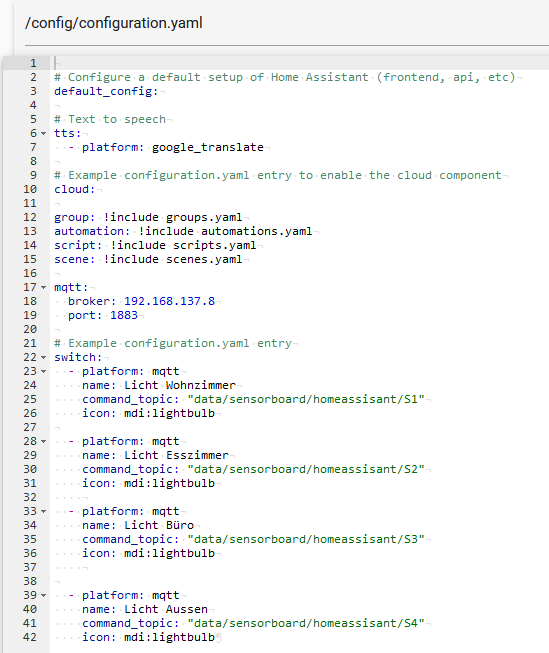
\includegraphics[width=0.75\textwidth]{graphics/Homeassostantconfig.PNG}
	\caption{Configfile Home Assistant} 	
	\label{pic: Configfile Home Assistant}
\end{figure}

\item Hinzu fügen von Schalter, welche mit Sprachbefehl Mqtt-Message generieren. Der Name des Schalters ist ebenso die Bezeichnung für den Sprachbefehl.
 \item In den 'Einstellungen' Home Assistant Cloud anmelden, Konto erstellen. Mit Google Home App  auf Smartphone mit 'Gerät verbinden', Home Assistant wählen und mit Cloud Benutzerkonto anmelden.
 
\end{enumerate}

\subsection{Topics}
In Nachfolgenden Tabelle \ref{tab: MQTT-Topics Home Assistant} sind die vom Home Assistant generierten Topics, welche weiter in Openhab verwendet werden.
\begin{table}[H]
	\centering
	\begin{tabular}{|l|l|}
		\hline 
		Topic  & Funktion  \\ 
		\hline 
	data/sensorboard/homeassisant/S1 & Sprachbefehl von Google Assistant empfangen  \\ 
		\hline
	data/sensorboard/homeassisant/S2 & Sprachbefehl von Google Assistant empfangen \\ 
		\hline
	data/sensorboard/homeassisant/S3 & Sprachbefehl von Google Assistant empfangen \\ 
		\hline
		data/sensorboard/homeassisant/S4 & Sprachbefehl von Google Assistant empfangen  \\ 
		\hline
	\end{tabular} 	
	\caption{MQTT-Topics Home Assistant}
		\label{tab: MQTT-Topics Home Assistant}
\end{table}